\clearpage
\section{Results}
\label{sec:results}

In this section we present the results obtained by following the research tracks as explained in section \ref{sec:experimental-design}. We first evaluate the performance on the visual only model. Next, we evaluate which accelerometer based model performs best. Finally, we look at the performance after fusion both data sources.

% We first describe the results of the visual model. We also include the various tested configurations, and report on the best performing model. Then, we describe the various network architectures of the accelerometer model. 

\subsection{Track 1: Detecting Manholes with Visual Model}

As described section \ref{sec:track-1-design} we retrain YOLO to detect manholes. We evaluate with various configurations of network sizes, input image sizes, and including proportion of RDD dataset. 

\subsubsection{Iteration 1: Training YOLO}

In the first experiment of this track we evaluate the effect of the model size and the input size. The result summary are listed in table \ref{tab:results-yolo-v1}, and the Average Precision over each epoch is shown in \ref{fig:results-yolo-v1}. Note, the results are for the first iteration, i.e., training YOLO as object detection.

From these results we conclude that the model \code{v1\_s\_1280\_8} performs best. The Average Precision between this model, and the second best (\code{v1\_m\_1280\_4}) are close (0.484 for small vs 0.473 for medium). Although the latter model has a higher precision, its recall is lower and the running time is significantly longer. When detecting road anomalies it can be argued that a higher recall is preferred over precision.

From the results we see that training with larger network size doesn't guarantee better performance in this task. This is likely as detecting manholes is relatively easy for YOLO. Increasing the input size of the image does improve performance. We can see that both model sizes have higher performance when the input size is larger. This makes sense as more pixels are preserved with a higher input size.

Note, during experiments the batch size is set to the largest possible value without exceeding the available resources. As the author of YOLO recommends, too small batches should be avoided as it impacts the learning performance \cite{yolo-training-tips}. Unfortunately the current machine was not capable of training larger YOLO models or when increasing the input size.

% Please add the following required packages to your document preamble:
% \usepackage{graphicx}
\begin{table}[ht]
\centering

\begin{tabular}{|l|l|l|l|l|l|l|l|}
\hline
\textbf{Name}  & \textbf{Model Size} & \textbf{Input Size} & \textbf{Batch Size} & \textbf{Precision} & \textbf{Recall} & \textbf{AP} & \textbf{Runtime} \\ \hline
v1\_m\_1280\_4 & YOLOv5m             & 1280                & 4                   & 0.766              & 0.396           & 0.473       & 3h 46m           \\ \hline
v1\_m\_640\_16 & YOLOv5m             & 640                 & 16                  & 0.521              & 0.345           & 0.316       & 51m              \\ \hline
\textbf{v1\_s\_1280\_8} & YOLOv5s             & 1280                & 8                   & 0.622              & 0.465           & 0.484       & 1h 26m           \\ \hline
v1\_s\_640\_16 & YOLOv5s             & 640                 & 24                  & 0.512              & 0.245           & 0.298       & 36m              \\ \hline
\end{tabular}
\captionsetup{width=.90\textwidth}
\caption{Evaluation metrics of various YOLO configurations. From these results we conclude that the model \code{v1\_s\_1280\_8} performs best.}
\label{tab:results-yolo-v1}
\end{table}


\begin{figure}[ht]
\begin{center}
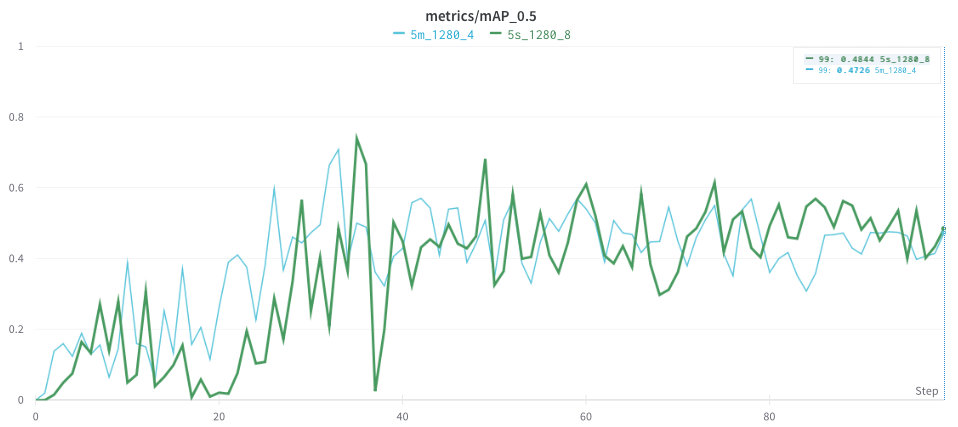
\includegraphics[height=5cm,keepaspectratio]{images/6_results/v1-yolo-map.png}
\end{center}
\captionsetup{width=.90\textwidth}
\caption{Graph showing the Average Precision for the two best models over each epoch.}
\label{fig:results-yolo-v1}
\end{figure}

In the next experiment, the model (\code{v1\_s\_1280\_8}) is further trained on additional data from the Road Damage Dataset (RDD) \cite{road-damage-detector}. From the RDD we select 80 random images (10\% of the training set) where a manhole is visible, and 40 random background images (5\% of the training set). Remember that the dataset is collected in different countries, therefore the manholes in those countries look different. To this aim, we evaluate if our model is able to learn from a more generalized dataset.

The results are shown in table \ref{tab:results-yolo-v2}. As we can see the performance of both models are very comparable after training for some while. Note, the model without RDD early stopped after training for 72 epochs. This is because the validation loss stopped declining, indicating that the model is saturated and does not learn further. From figure \ref{fig:results-yolo-v2}, we see that the model with RDD takes more epochs to reach comparable performance. However, with this dataset the model learns from a more generic dataset. 

\begin{table}[ht]
\centering
\begin{tabular}{|l|l|l|l|l|l|}
\hline
\textbf{Name}    & \textbf{Epochs} & \textbf{Precision} & \textbf{Recall} & \textbf{AP} & \textbf{Runtime} \\ \hline
v2\_with\_rdd    & 100             & 0.752              & 0.599           & 0.649       & 2h 56m           \\ \hline
v2\_without\_rdd & 72              & 0.746              & 0.610           & 0.644       & 1h 4m            \\ \hline
\end{tabular}
\captionsetup{width=.90\textwidth}
\caption{Evaluation metrics of augmenting the training }
\label{tab:results-yolo-v2}
\end{table}

\begin{figure}[ht]
\begin{center}
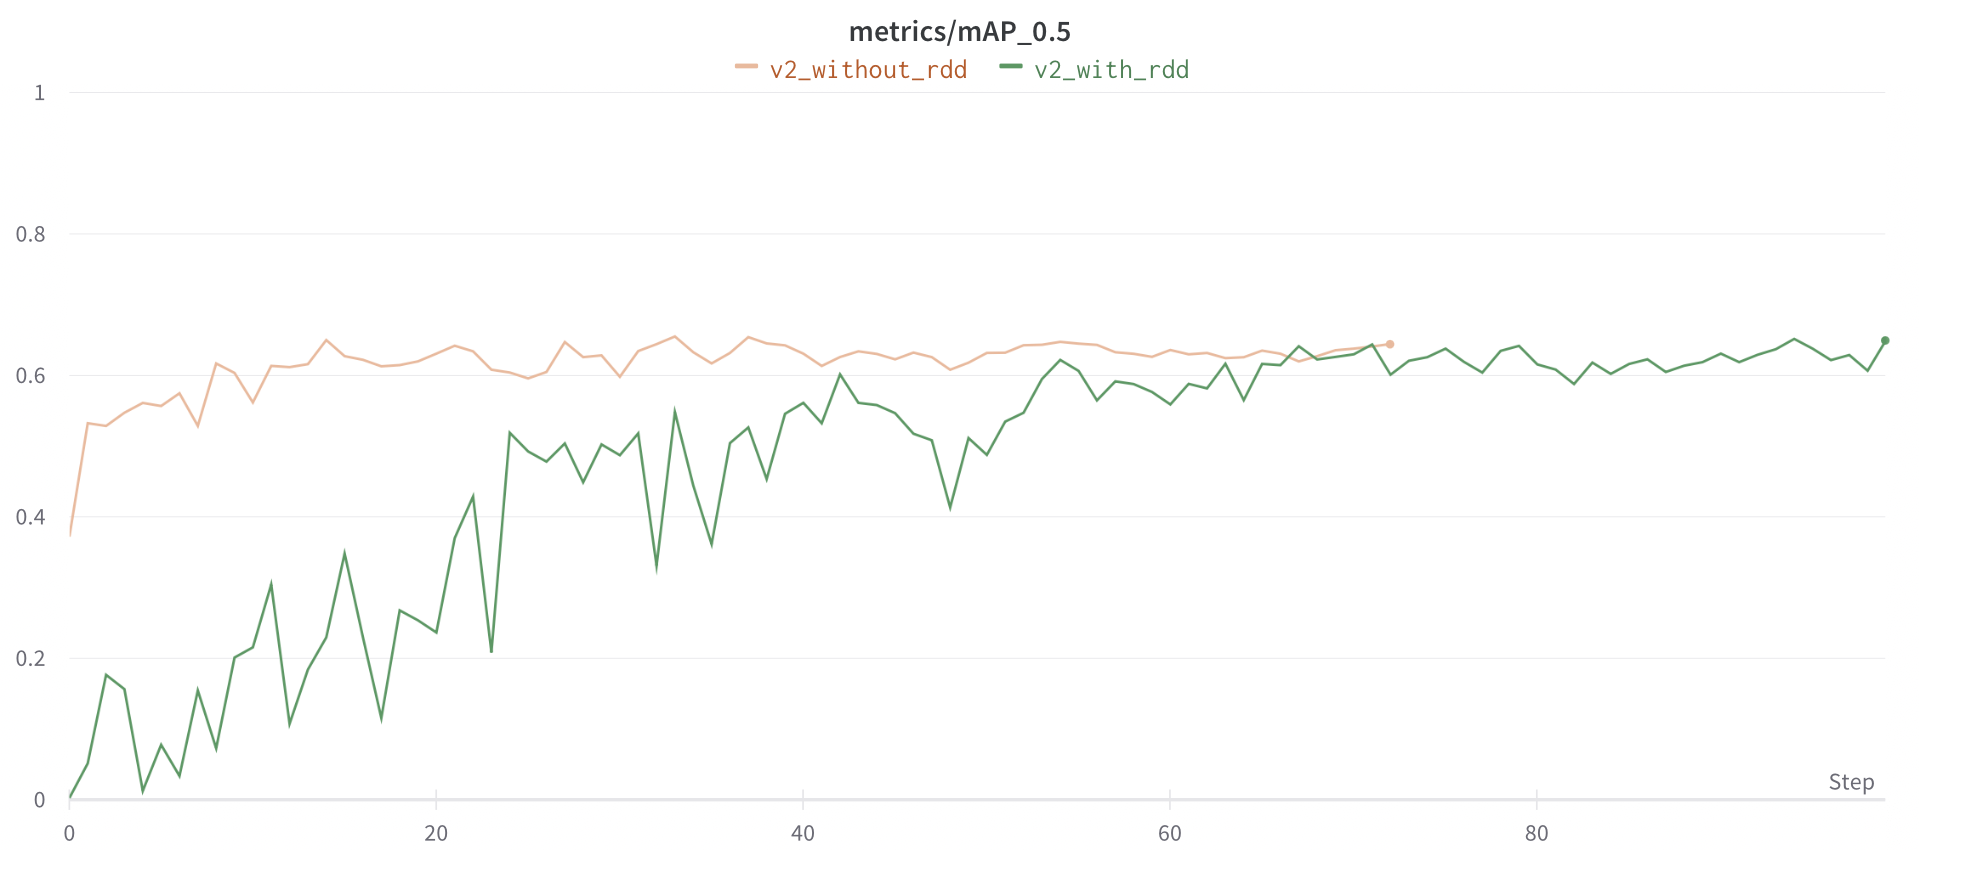
\includegraphics[height=5cm,keepaspectratio]{images/6_results/v2-yolo-rdd.png}
\end{center}
\captionsetup{width=.90\textwidth}
\caption{Graph showing the Average Precision for the two best models over each epoch.}
\label{fig:results-yolo-v2}
\end{figure}


\subsubsection{Iteration 2: Modifying to Binary Classification}

In the second iteration, we modify the best YOLO configuration. We replace the object detection head with a head capable of binary classification. This makes the model suitable for comparison with the models developed in other tracks. The model \code{v1\_s\_1280\_8} is used as a base. As we found that supplementing the dataset with RDD did not yield significant improvements.

The model is modified as described in section \ref{sec:yolo}. The layers of the YOLO model are kept frozen, i.e., the parameters are kept and not further trained. The final layers of the model are trained on the segmented dataset to perform classification. This makes the learning task of the model easy. The model is trained for only 20 epochs. The batch size of the model is configured to be 1. Higher batch sizes causes memory errors.

The training results can be seen in the plots of figure \ref{fig:results-visual-plots} and in table \ref{tab:results-visual-plots}. The top-left shows the loss over epoch. After 20 epochs, we can see that the training and validation loss are both low. This indicates that the model learned sufficiently and is neither over- or underfitting. This is also confirmed by the top-right plot. Here is shown the Precision Recall curve. The model has a perfect performance. This confirms that the learning task of making classifications is easy for the model.


\begin{table}[ht]
\centering
\begin{tabular}{|l|l|l|l|l|}
\hline
\textbf{Model} & \textbf{Precision} & \textbf{Recall} & \textbf{AP} & \textbf{F1} \\ \hline
Visual Only & 0.86               & 1.0             & 1.0         & 0.93        \\ \hline
\end{tabular}
\captionsetup{width=.90\textwidth}
\caption{Evaluation summary of the visual model.}
\label{tab:results-visual-plots}
\end{table}


\begin{figure}[ht]
\begin{center}
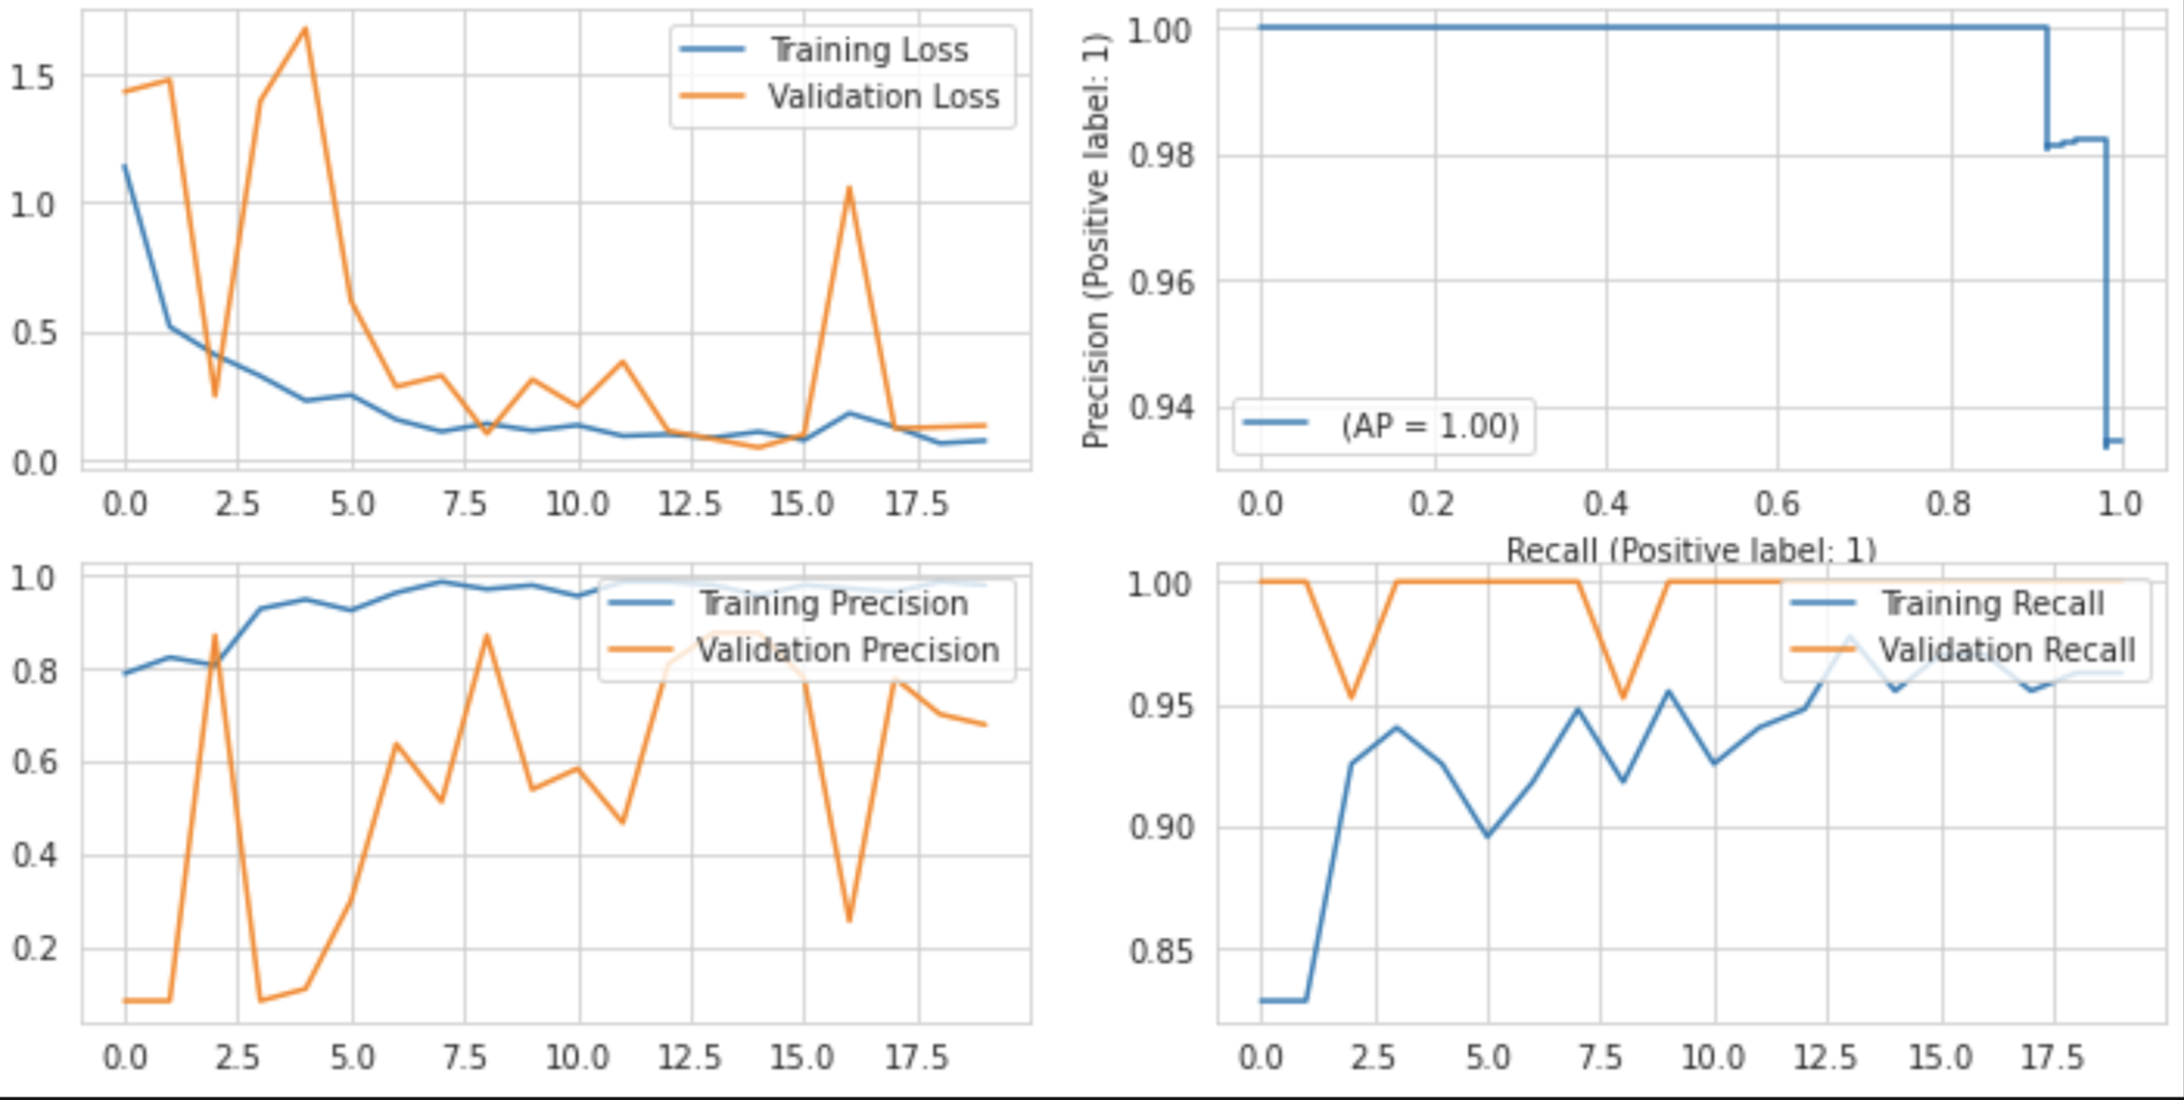
\includegraphics[width=.80\textwidth,keepaspectratio]{images/6_results/visual-learning.png}
\end{center}
\captionsetup{width=.90\textwidth}
\caption{Showing various plots of the learning performance of the visual only model. In the top-left is the training and validation loss over each epoch. In the top-right the precision recall curve for the test set. The bottom plots show the precision and recall over each epoch.}
\label{fig:results-visual-plots}
\end{figure}


\subsubsection{Conclusion}

After iteration 2, we developed a model capable of classifying whether a segment contains a manhole. This model performs really well on the test set. This is attributed due the YOLO model. As YOLO is currently state-of-the-art in object detection, making classifications is relatively easy task.


\subsection{Track 2: Detecting Manholes with Accelerometer Data}

As described in section \ref{sec:track-2-design} we train various models using accelerometer data. The input to the models is either the raw accelerometer data, or after performing Fourier transform. During this track we evaluate three network architectures: Dense Neural Network, Convolutional Neural Network, and LSTM Network. In total this means we train and evaluate 6 different machine learners.

Each model is optimized using Adam with learning rate of $0.001$. The model is trained for 100 epochs, and restored to the best weights before evaluating test scores. To this aim we achieve better generalization in case the model overfits on the training set \cite{Goodfellow2016}. The results can be found in table \ref{tab:results-acc}. The reported statistics are calculated on the held out test set. Note, the threshold for positive prediction are all kept constant at $0.5$ for a equivalent comparison.

In general, we see that all model architectures perform better on the raw accelerometer data instead after applying feature extraction. It can be seen that the CNN models outperform the other models. This is followed by the LSTM network operating on raw data. Finally, the DNN based model performs relatively poorly. Next we dive into the specific learning performance for each model. As all models operating on the raw data performs better, we only report on the raw version.


\begin{table}[ht]
\centering
\begin{tabular}{|l|l|l|l|l|}
\hline
\textbf{Name} & \textbf{Precision} & \textbf{Recall} & \textbf{AP} & \textbf{F1} \\ \hline
\textbf{CNN (raw)}      & 0.29               & 1.0             & 0.51        & 0.45        \\ \hline
LSTM (raw)     & 0.39               & 0.95            & 0.48        & 0.55        \\ \hline
Dense (raw)    & 0.28               & 0.77            & 0.34        & 0.41        \\ \hline
CNN (FFT)      & 0.28               & 0.95            & 0.51        & 0.44        \\ \hline
LSTM (FFT)     & 0.31               & 0.89            & 0.25        & 0.46        \\ \hline
Dense (FFT)    & 0.36               & 0.42            & 0.41        & 0.39        \\ \hline
\end{tabular}
\captionsetup{width=.90\textwidth}
\caption{Evaluation summary of the various machine learning models.}
\label{tab:results-acc}
\end{table}


\begin{minipage}{\textwidth}
\subsubsection{Dense Neural Network}

In figure \ref{fig:results-acc-dense} we see the learning performance. As could be seen earlier in the table, the DNN model does not yield great performance. Especially lacking is the recall of the model. From the top-left plot we can see that the model learns from the data. After epoch 50 starts overfitting. This is indicated as the validation loss keeps increasing with further epochs.
\vskip 1\baselineskip

\begin{center}
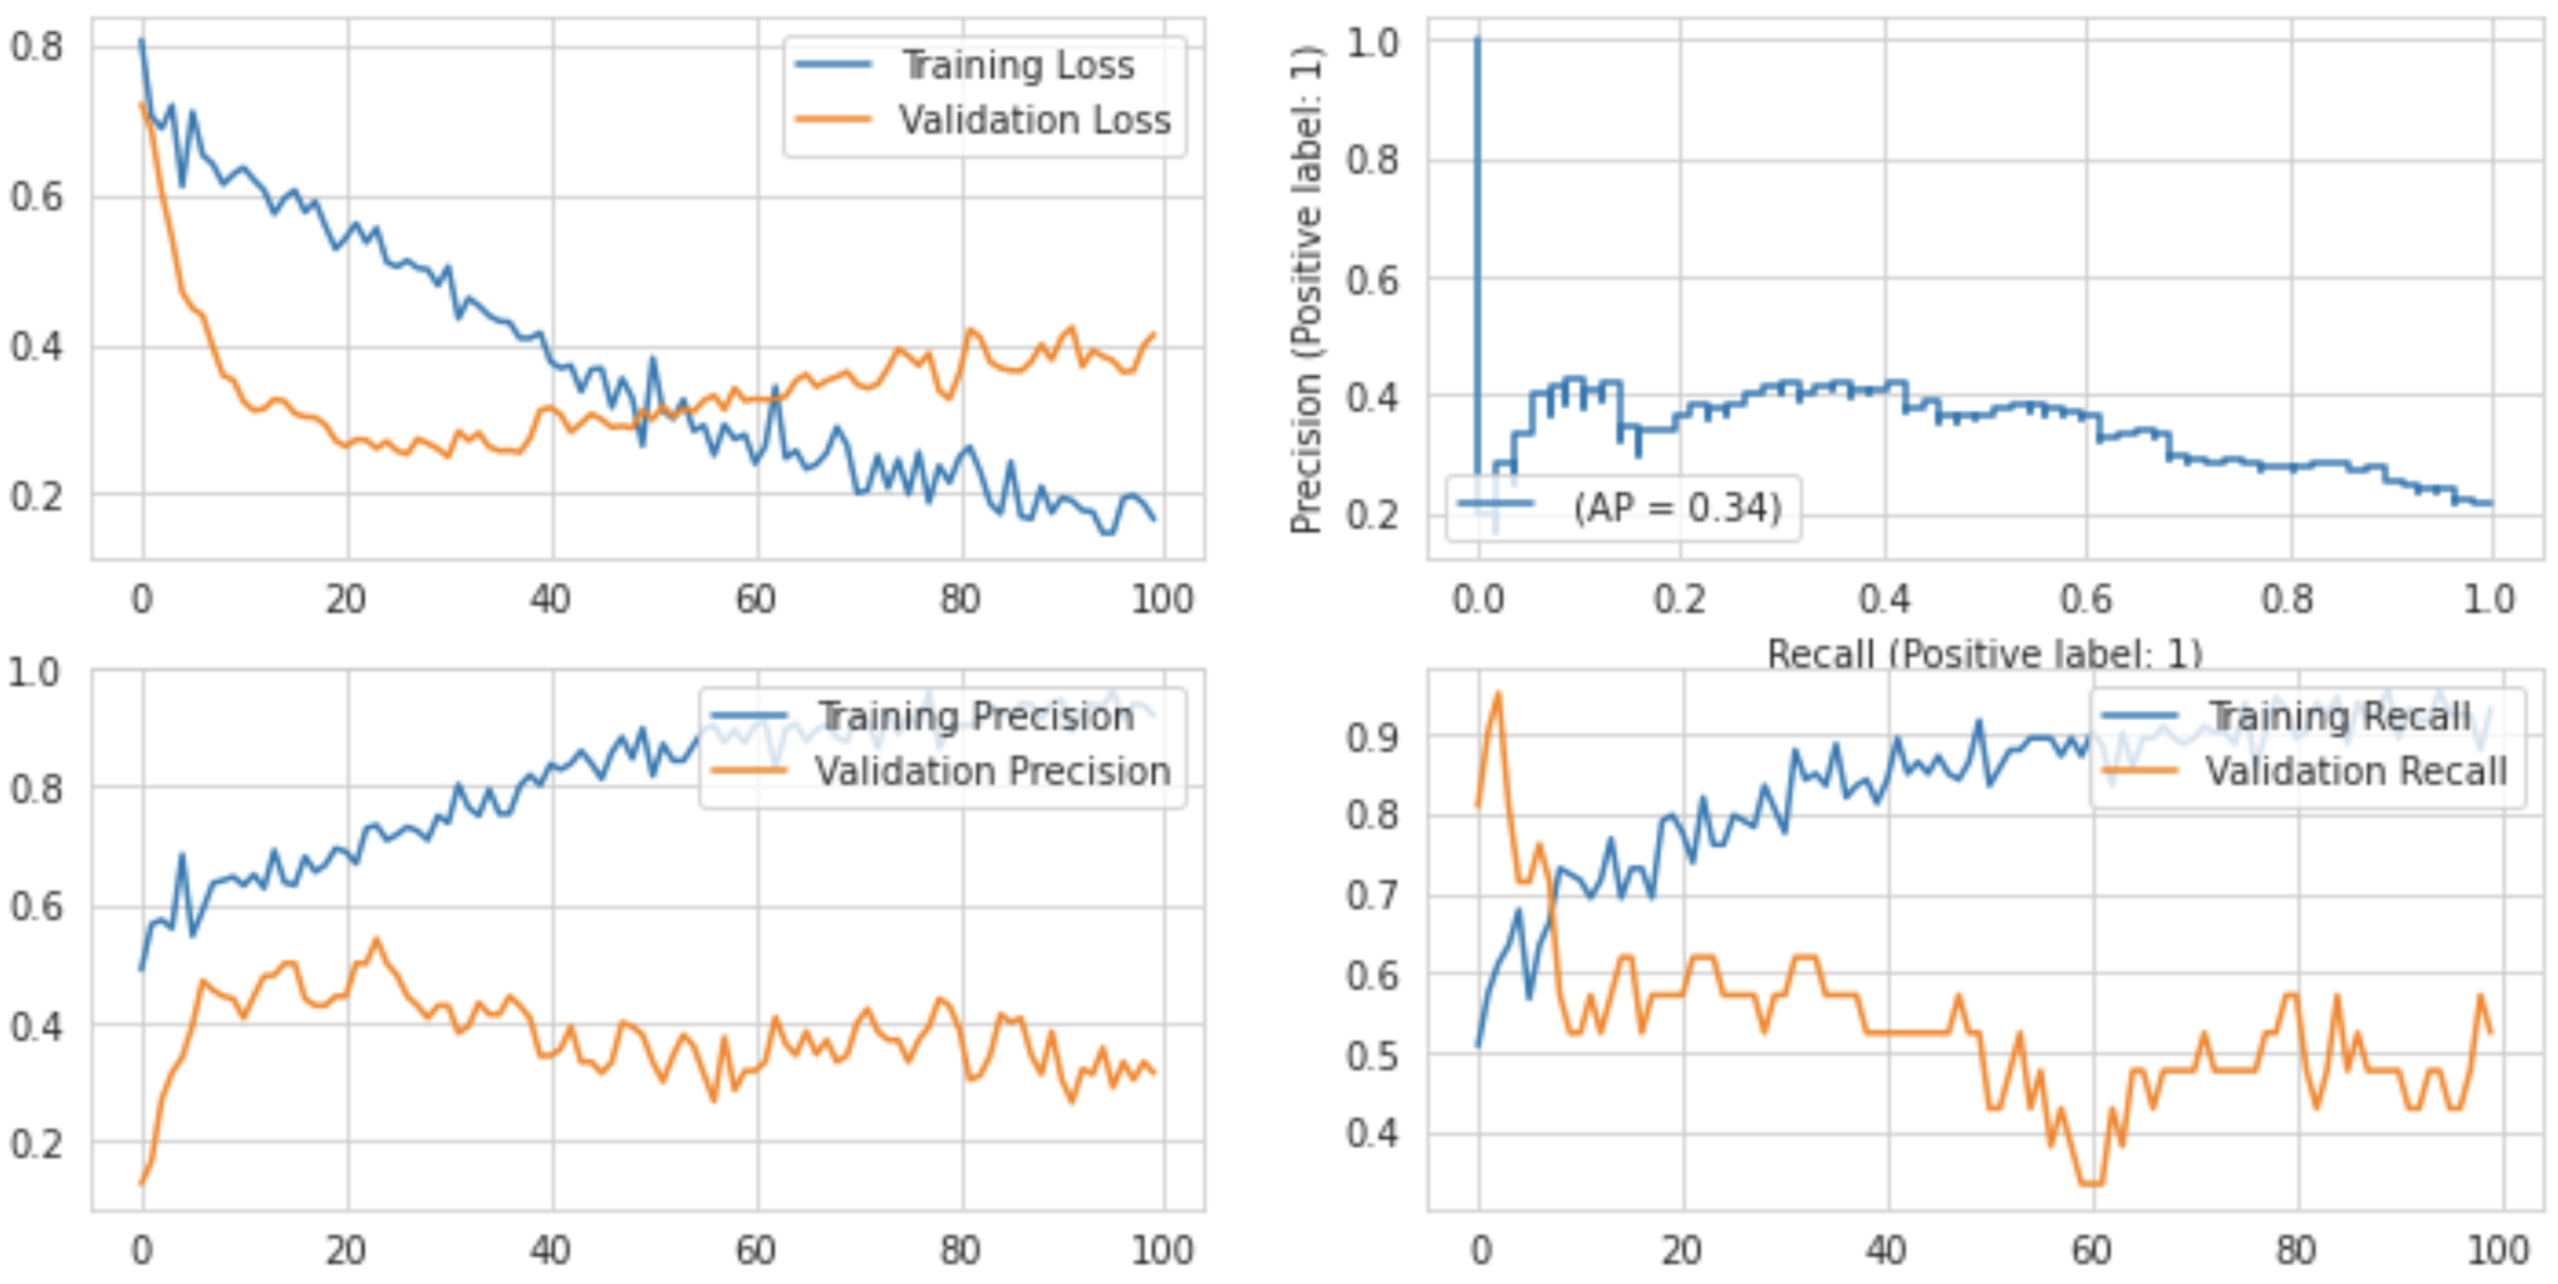
\includegraphics[width=.75\textwidth,keepaspectratio]{images/6_results/results-acc-dense.png}
\end{center}
\captionsetup{width=.90\textwidth}
\captionof{figure}{Showing various plots of the learning performance of the DNN accelerometer only model. In the top-left is the training and validation loss over each epoch. In the top-right the precision recall curve for the test set. The bottom plots show the precision and recall over each epoch.}
\label{fig:results-acc-dense}
\vskip 1\baselineskip
\end{minipage}

\begin{minipage}{\textwidth}
\subsubsection{Convolutional Neural Network}

From the accelerometer based models, the CNN performs best. The learning performance is shown in figure \ref{fig:results-acc-cnn}. Again the model shows sign of overfitting after epoch 50. This can be attributed due the high recall rate. However, this might indicate that this model is affected due the imbalanced dataset. Regardless, from the evaluation on the test set in the precision recall curve, we see acceptable performance. At recall rate of 0.8, the model evaluated with a precision of almost 0.7. 
\vskip 1\baselineskip

\begin{center}
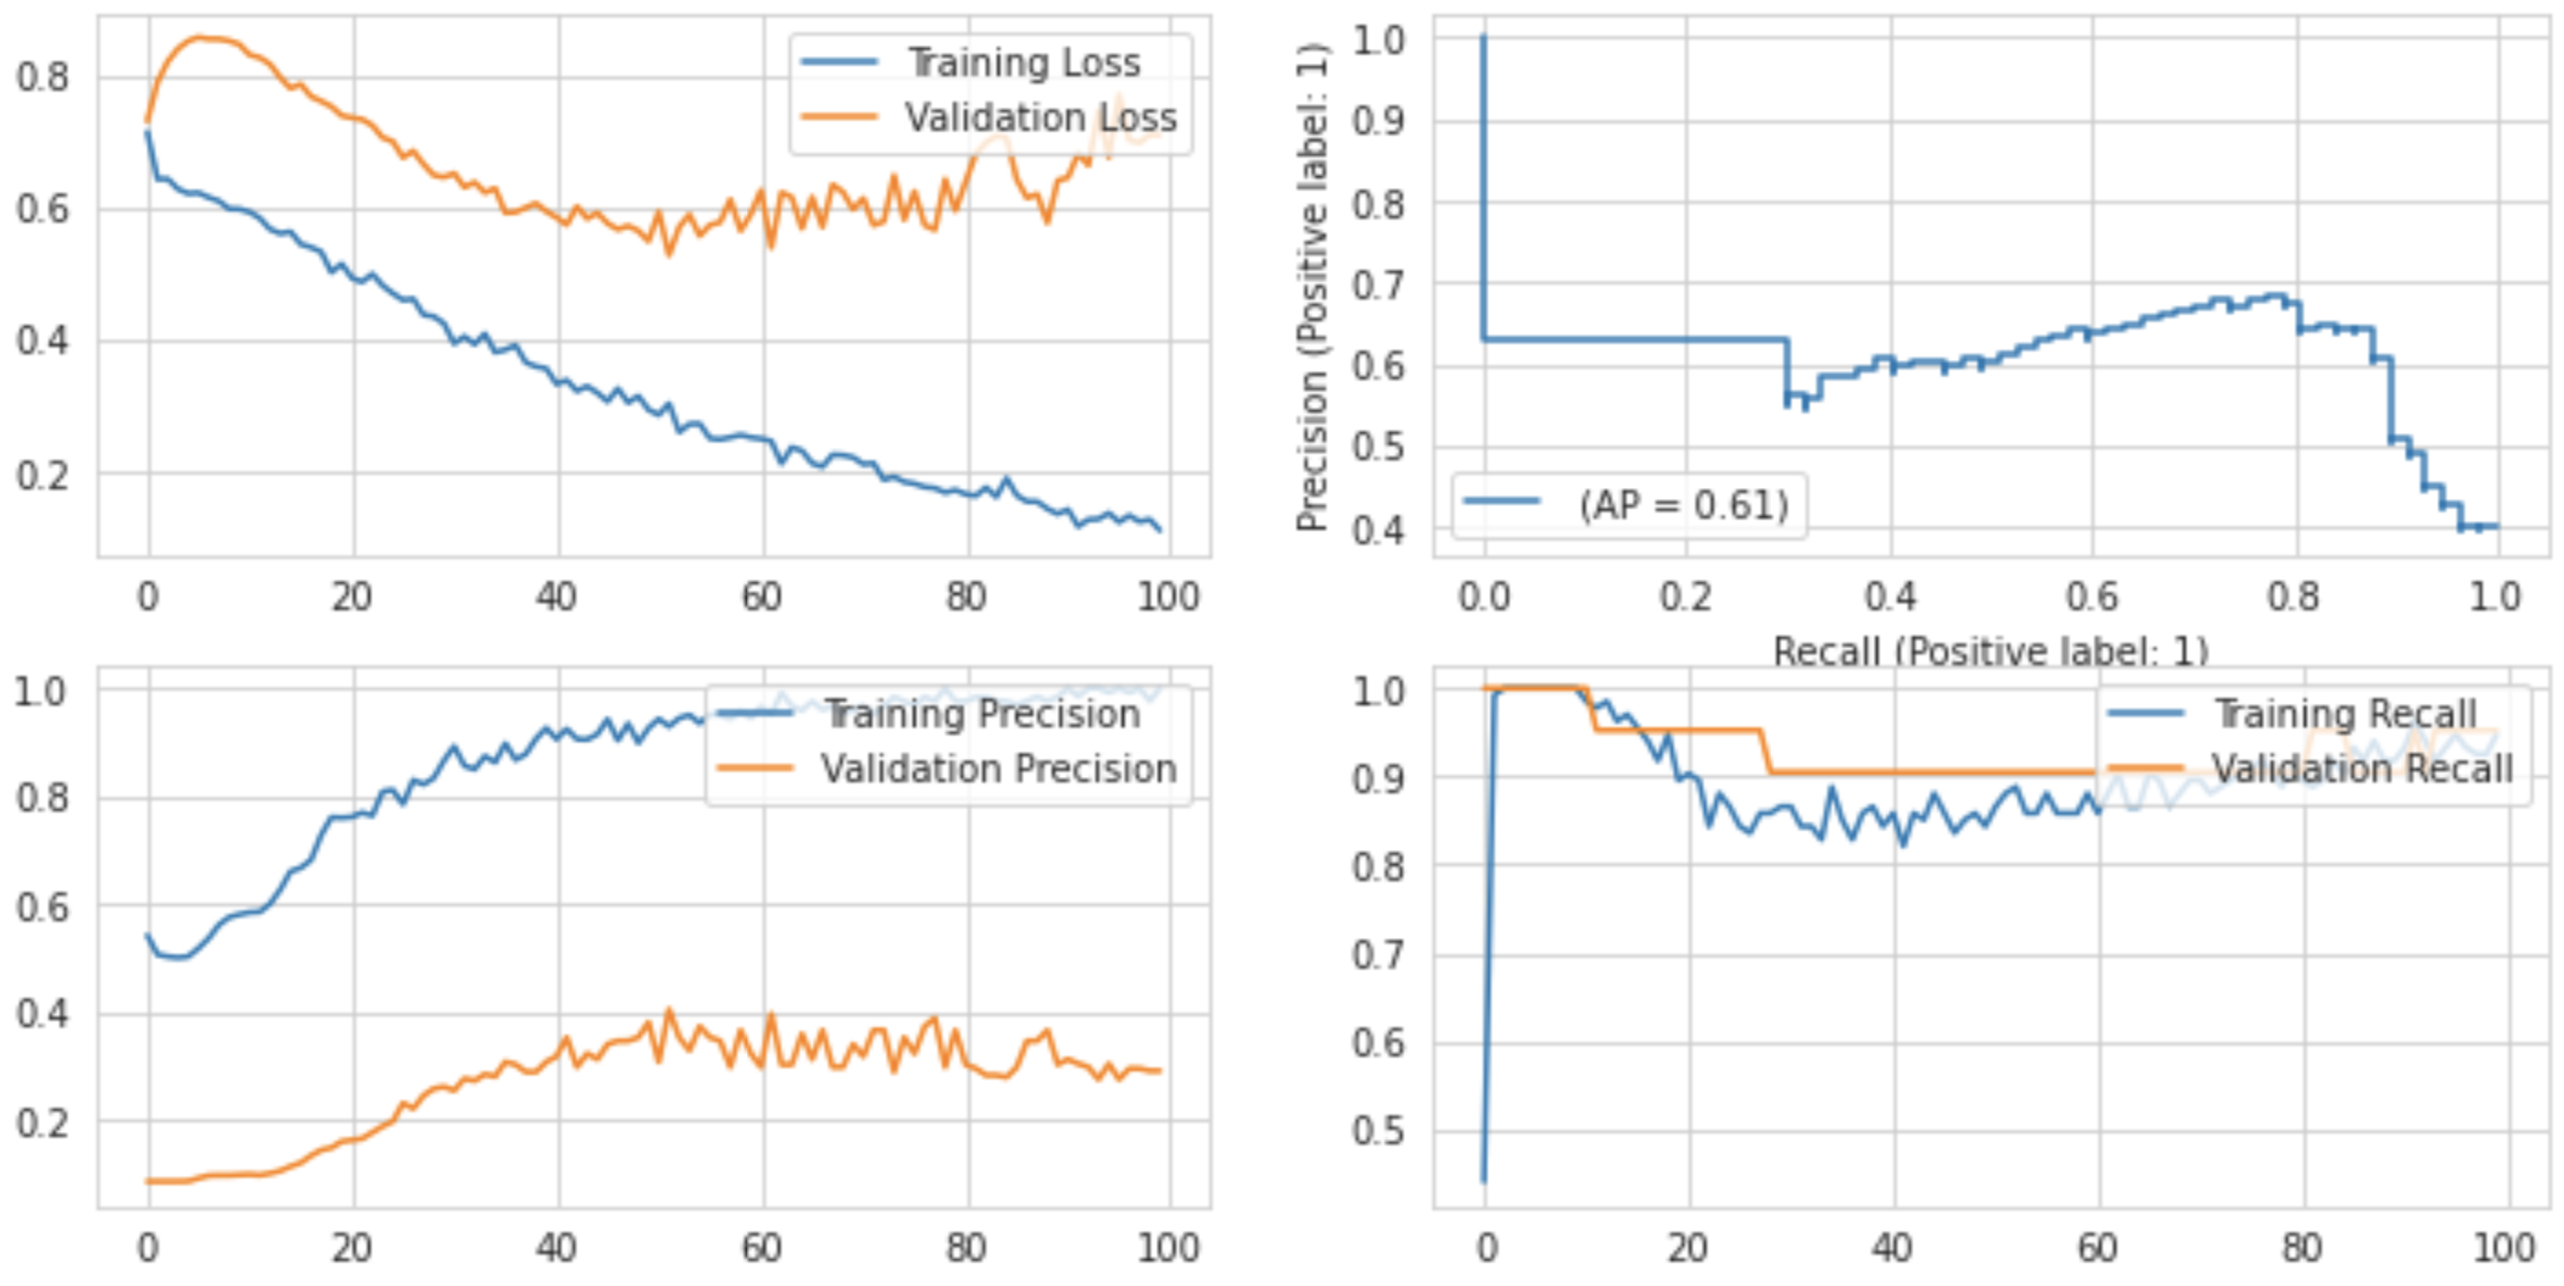
\includegraphics[width=.75\textwidth,keepaspectratio]{images/6_results/results-acc-cnn.png}
\end{center}
\captionsetup{width=.90\textwidth}
\captionof{figure}{Showing various plots of the learning performance of the CNN model. In the top-left is the training and validation loss over each epoch. In the top-right the precision recall curve for the test set. The bottom plots show the precision and recall over each epoch.}
\label{fig:results-acc-cnn}
\vskip 1\baselineskip
\end{minipage}

\begin{minipage}{\textwidth}
\subsubsection{LSTM Neural Network}

Finally we have the LSTM based model, see figure \ref{fig:results-acc-lstm}. This model scores second best, but from the top-left loss plots we see that this model quickly overfits. Additionally, due the spikes in the validation loss, we observe that this model is not training very well. The precision recall curve shows a relative flat curve. However, the overal precision of the model is underperforming with that of the CNN based model.
\vskip 1\baselineskip

\begin{center}
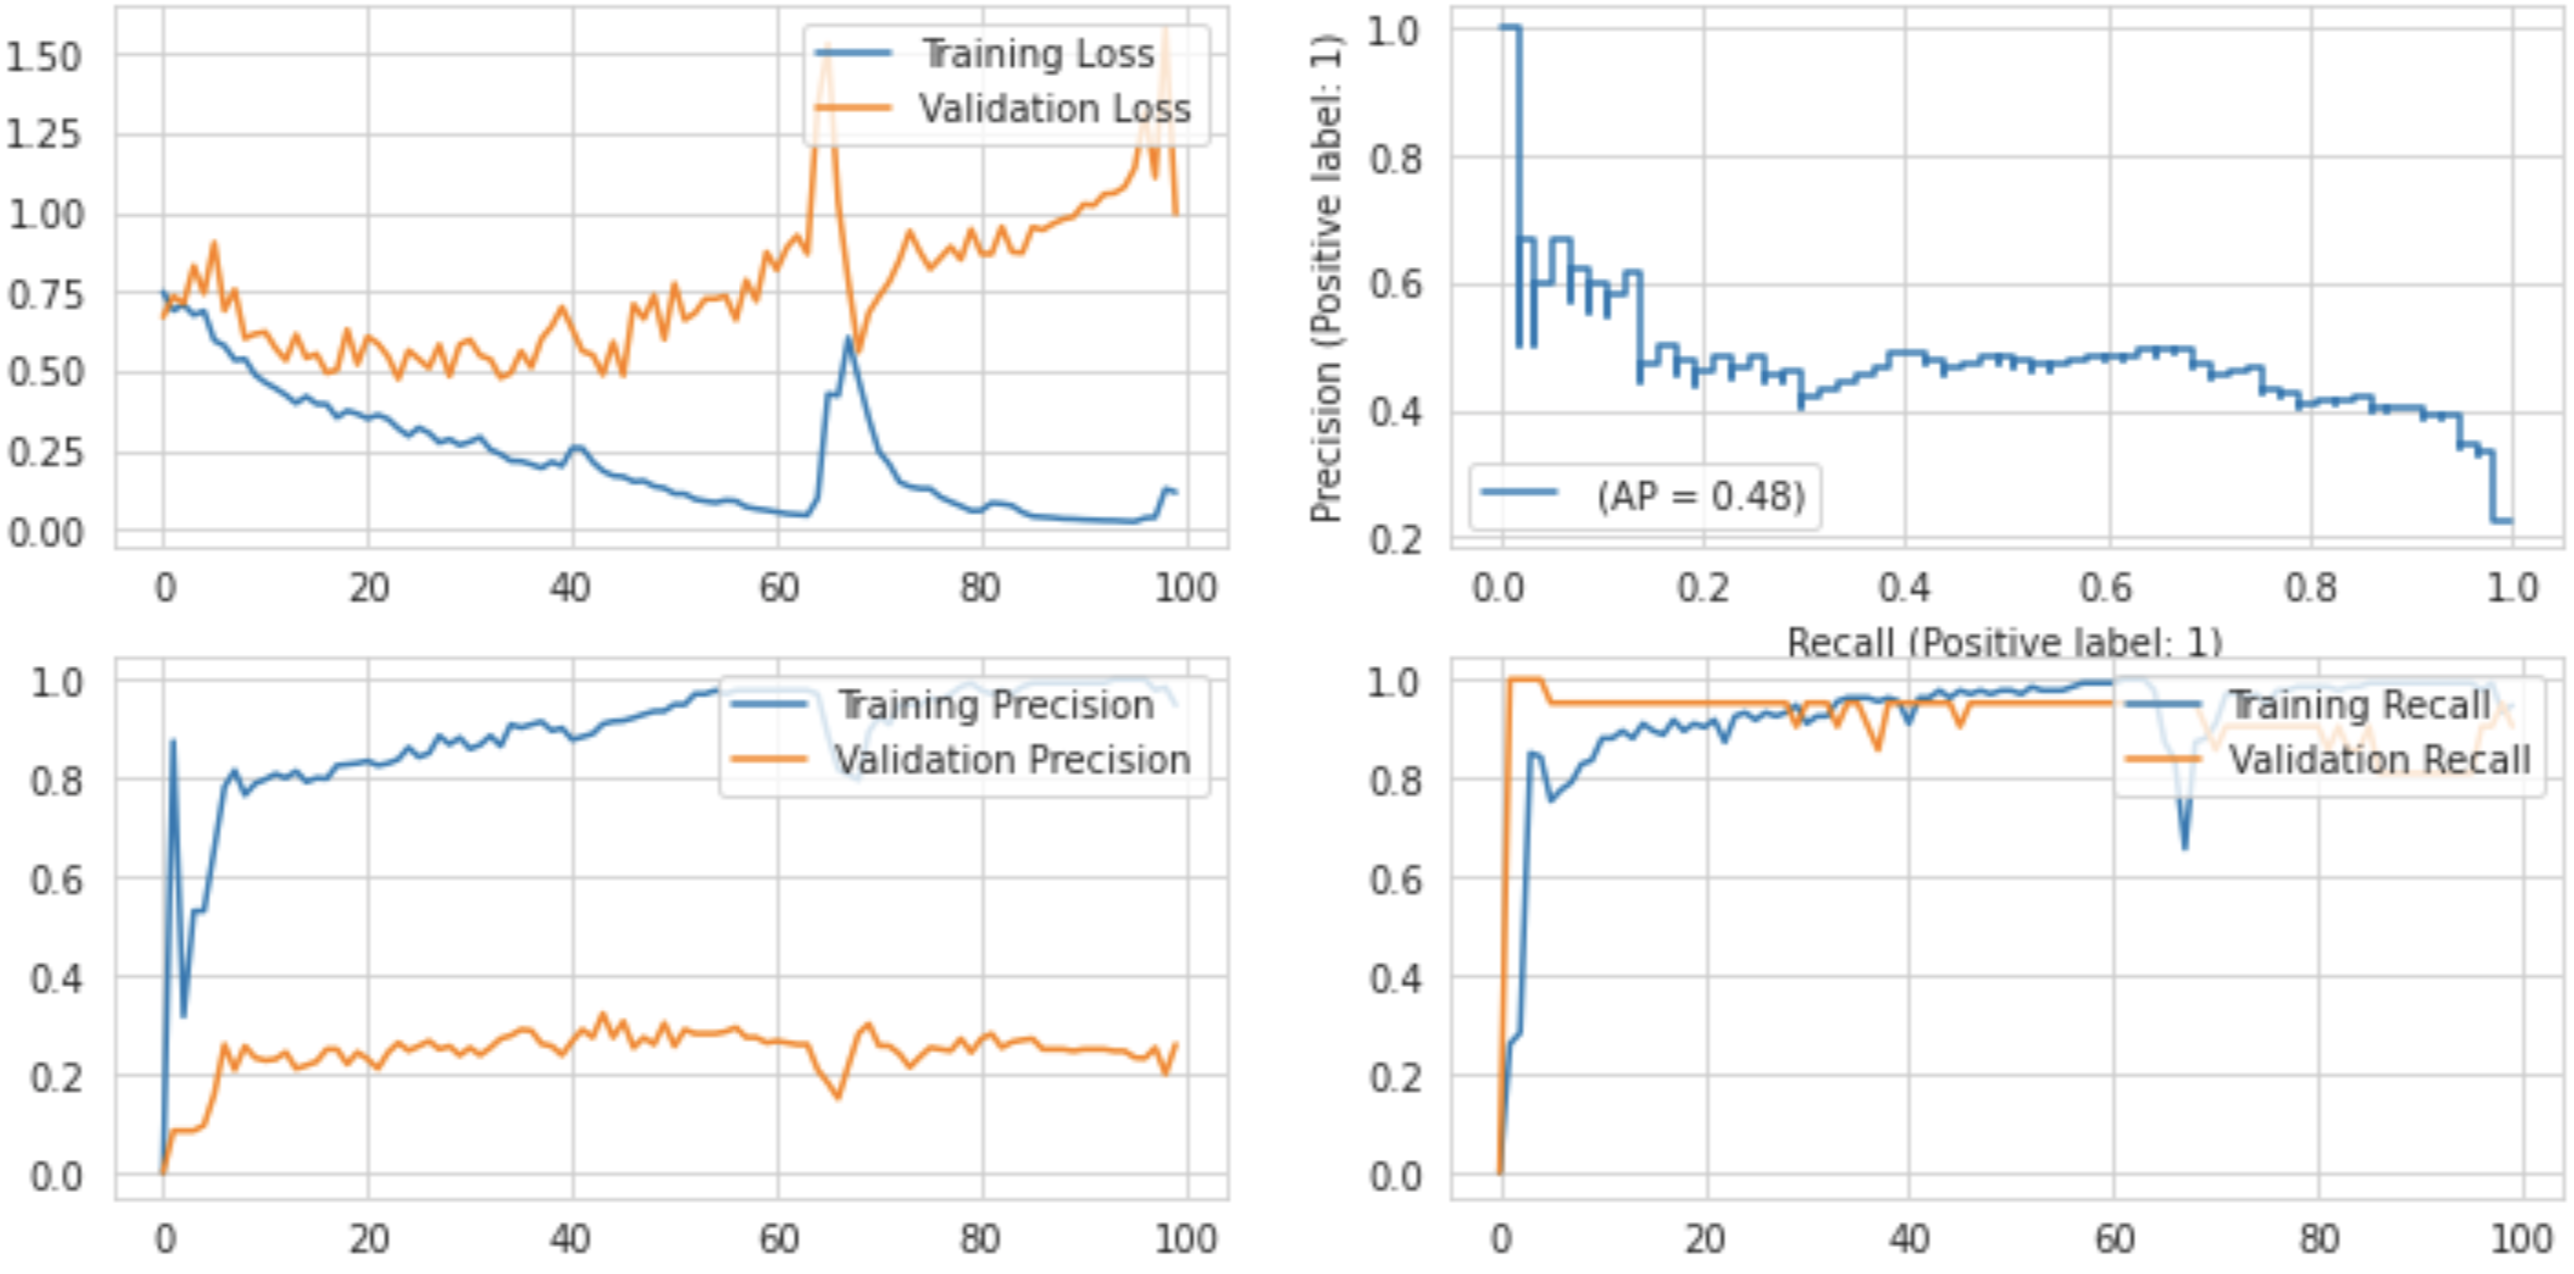
\includegraphics[width=.75\textwidth,keepaspectratio]{images/6_results/results-acc-lstm.png}
\end{center}
\captionsetup{width=.90\textwidth}
\captionof{figure}{Showing various plots of the learning performance of the LSTM model. In the top-left is the training and validation loss over each epoch. In the top-right the precision recall curve for the test set. The bottom plots show the precision and recall over each epoch.}
\label{fig:results-acc-lstm}
\end{minipage}

\subsubsection{Conclusion}

From the summary table we see that the precision and recall scores are relatively close for the CNN and LSTM based model. However, the Average Precision (AP) of the CNN model is significantly higher. This is also confirmed when comparing the respective Precision-Recall curves, see figure \ref{fig:results-acc}. The figure confirms that the CNN model (orange line) is able to make more accurate predictions at higher recall rates. This is indicated as the precision remains high, while the recall increases.

From the results we conclude that the CNN model without feature extraction performs best. We use this model in the following section, where we combine both visual and accelerometer data.

\begin{figure}[ht]
\begin{center}
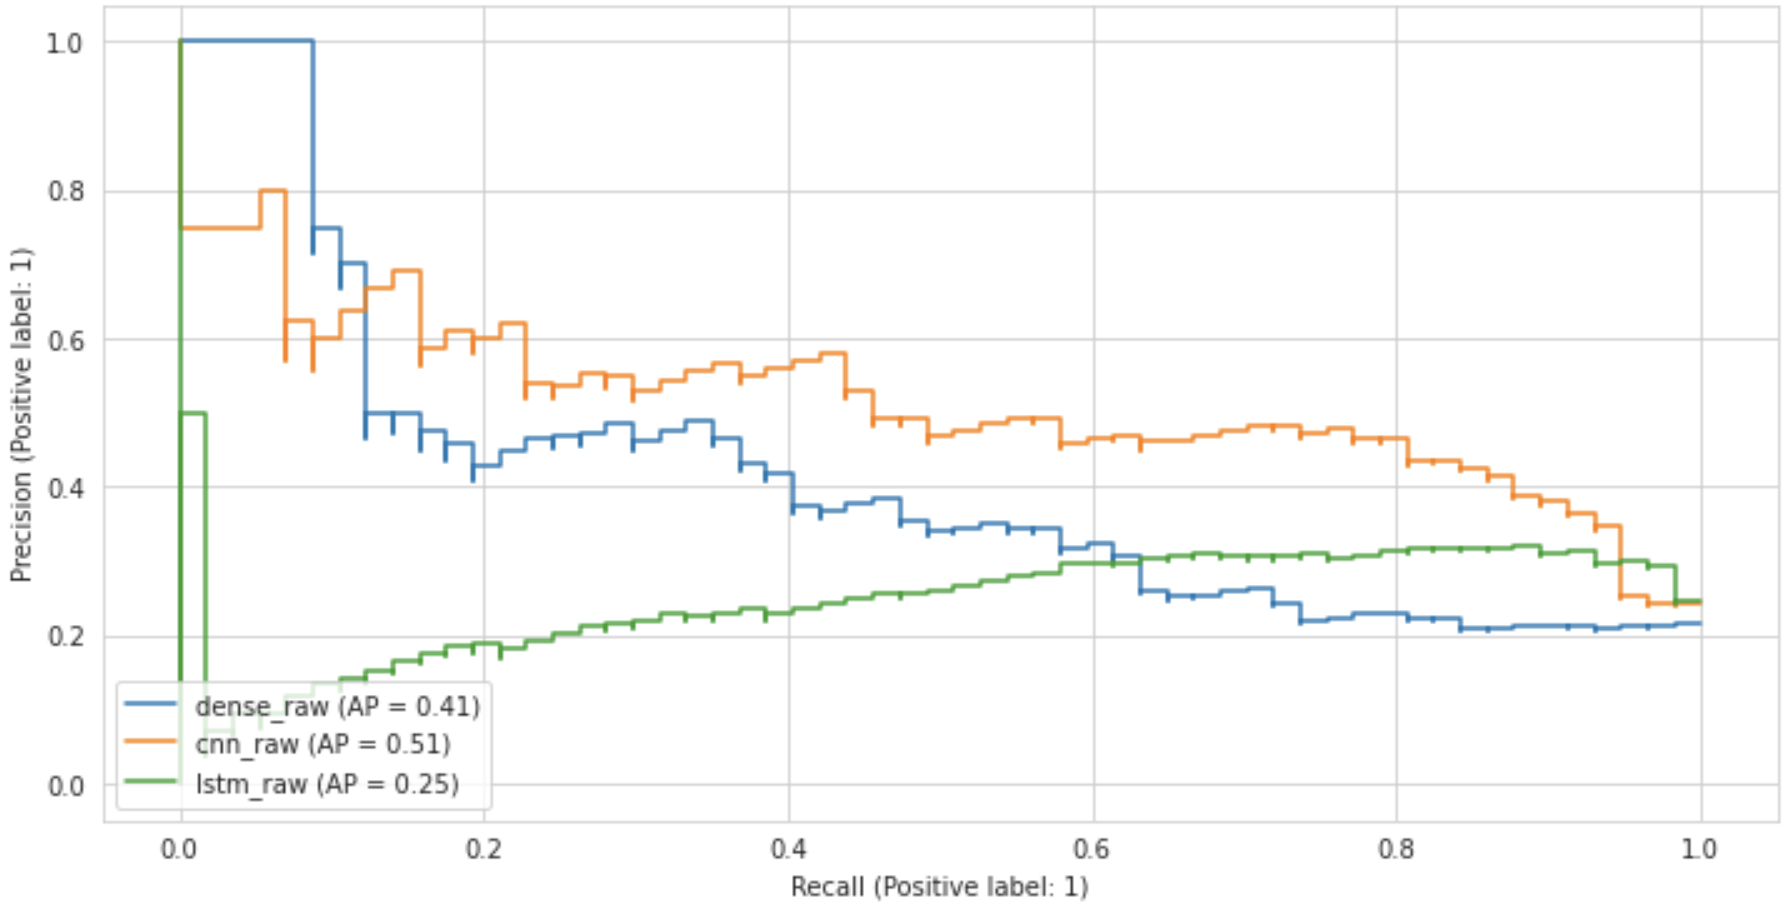
\includegraphics[width=.75\textwidth,keepaspectratio]{images/6_results/acc-prc.png}
\end{center}
\captionsetup{width=.90\textwidth}
\caption{This figure plots the Precision Recall Curve for each of the evaluated network architectures. For clarity only the models operating on raw input are shown.}
\label{fig:results-acc}
\end{figure}


\subsection{Track 3: Detecting Manholes with Multimodal Machine Learning}

In the final track, we combine the earlier developed unimodal models. As described in section \ref{sec:track-3-design}, this is done with both hybrid and late fusion. The results can be seen in table \ref{tab:results-fusion}. For comparison, the performance metrics are repeated of the unimodal models.

From table we can see that all models have a perfect recall of one. This means that all models are always able to identify all positives samples. The models vary in their precision. Unfortunately, the fusion based models do not outperform the unimodal models. The best performing model is that of the visual only model. 


\begin{table}[ht]
\centering
\begin{tabular}{|l|l|l|l|l|l|}
\hline
\textbf{Name}      & \textbf{Precision} & \textbf{Recall} & \textbf{AP} & \textbf{F1} & \textbf{Parameters} \\ \hline
\textbf{Visual Only}        & 0.86               & 1.0             & 1.0         & 0.93        & 7,566,817  \\ \hline
Accelerometer Only & 0.29               & 1.0             & 0.61        & 0.45        & 35,393     \\ \hline
Hybrid Fusion      & 0.66               & 1.0             & 0.88        & 0.79        & 7,602,144  \\ \hline
Late Fusion        & 0.62               & 1.0             & 1.0         & 0.77        & 7,602,210  \\ \hline
\end{tabular}
\caption{Evaluation metrics on the test set as reported by the respective models.}
\label{tab:results-fusion}
\end{table}

The hybrid fusion model adds layers to the network to combine both data sources. These layers are trained for 20 epochs using Adam optimizer with learning rate of 0.001. To this aim, we train a model which learns how to combine both data sources. The learning performance of the hybrid fusion model in figure \ref{fig:dense-network}. Related to the visual based model we observe that the model quickly starts to overfit. Regardless, the model as a good performance. The precision recall curve indicates a good fit.

\begin{figure}[ht]
\begin{center}
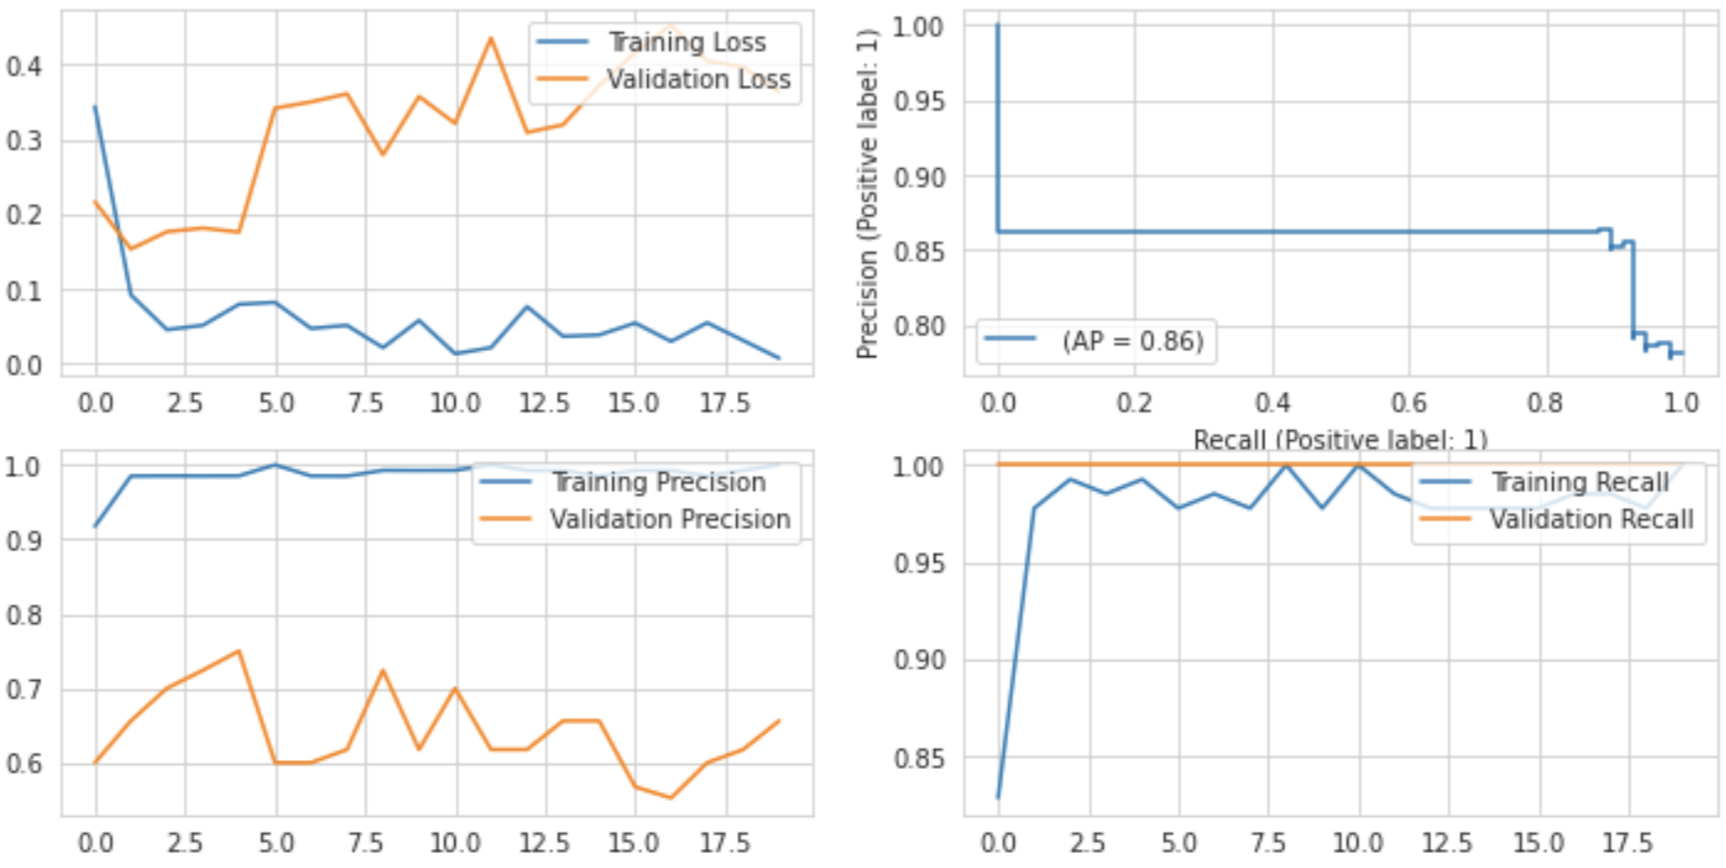
\includegraphics[width=0.75\textwidth]{images/6_results/results-hybrid-fusion.png}
\captionsetup{width=0.90\textwidth}
\captionof{figure}{Showing various plots of the learning performance of the hybrid fusion model. In the top-left is the training and validation loss over each epoch. In the top-right the precision recall curve for the test set. The bottom plots show the precision and recall over each epoch.}
\label{fig:dense-network}
\end{center}
\end{figure}


The late fusion model works by combining both unimodal representations after each respective model has made a decision. The final decision is made by a voting classifier. In this case, we average both probabilities. When it exceeds the threshold of 0.5, we classify the output as positive. This means that the model does not learn a joint representation. Therefore, we cannot report further results on this model except the reported statistics in table \ref{tab:results-fusion}.

% However, this is probably an effect of our dataset. It is imbalanced, and relatively low. Regardless, we argue that a high recall is preferred when detecting road surface anomalies.

% This likely because the accelerometer data are labelled according a heuristic.

% The best performing model is the visual only model.

% The model performances do vary in terms of precision. 

% From this table we see that the accelerometer based model performs poorly in terms of precision. This is probably due the partial observability as mentioned earlier in section \ref{}. Regardless, this effect is propagated in the multimodal models. The precision of the hybrid and late fused models are significantly lower than that of the visual model. 

\subsubsection{Evaluation on Single Input}

To test if the hybrid fused model actually learns a joint representation, we evaluate the performance when one of the inputs is zeroed out. This experiment is performed for both zeroing out the visual and the accelerometer data. The results are shown in table \ref{tab:results-fusion-compare}.

We can see from the results that the model still works when either input is zeroed out. This confirms that the model is able to learn a joint representation. Interestingly is that the model performance increases when only visual data is provided.

\begin{table}[ht]
\centering
\begin{tabular}{|l|l|l|l|l|}
\hline
\textbf{Name}                         & \textbf{Precision} & \textbf{Recall} & \textbf{AP} & \textbf{F1} \\ \hline
Hybrid Fusion with Both Inputs      & 0.66               & 1.0             & 0.88        & 0.79          \\ \hline
Hybrid Fusion with Visual Only        & 0.90               & 1.0             & 1.0         & 0.95        \\ \hline
Hybrid Fusion with Accelerometer Only & 0.68               & 0.77            & 0.61        & 0.72        \\ \hline
\end{tabular}
\caption{Evaluation of the hybrid fusion model where either both or each of the respective unimodal sources is provided.}
\label{tab:results-fusion-compare}
\end{table}

\subsubsection{Conclusion}

From the results we conclude that both multimodal fusions work. Admittedly, we see that that the unimodal vision only model performs best. This implies that the accelerometer data is not well prepared. We discuss this further in the following section.

In figure \ref{fig:example-classifications}, a matrix is shown where each model predicts the classification based on the input. Each image is a frame from the respective segment. For each image is shown the annotated label, and for each model the prediction outcome.


\begin{figure}[t]
\begin{center}
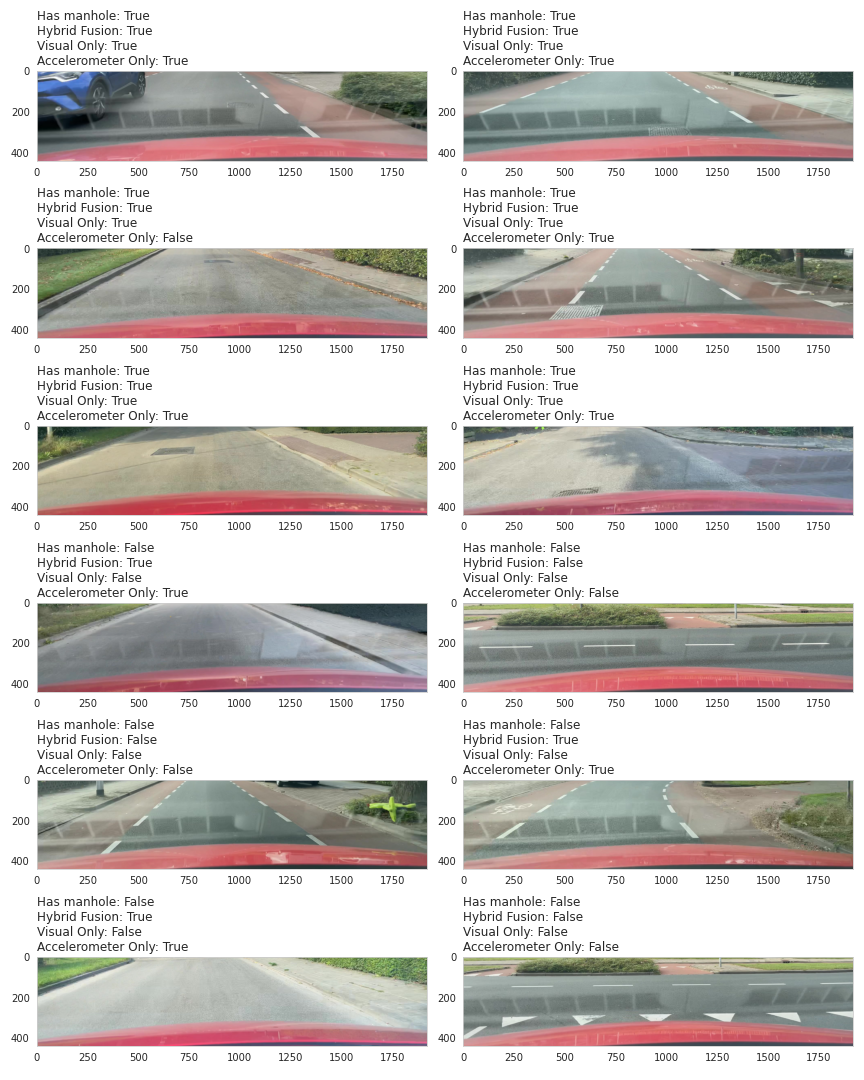
\includegraphics[width=\textwidth]{images/6_results/example-predictions-2.png}
\captionsetup{width=0.90\textwidth}
\captionof{figure}{Matrix of prediction examples.}
\label{fig:example-classifications}
\end{center}
\end{figure}